\subsection{Network and observation campaign}
\label{sec:results-network}

\begin{figure}[t]
  \centering
  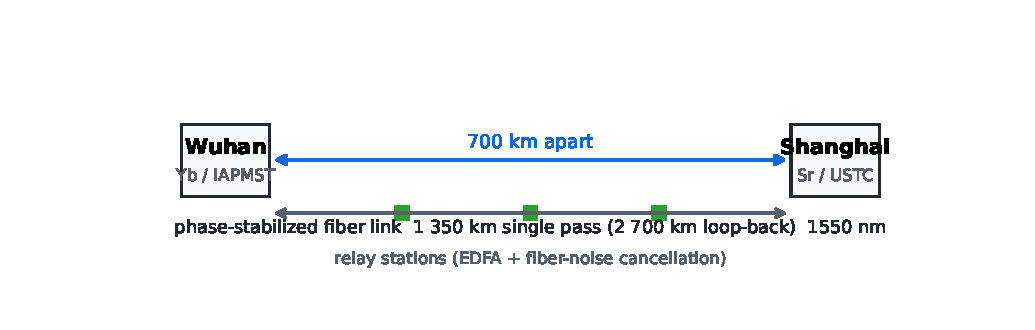
\includegraphics[width=\linewidth]{figs/fig1_network.pdf}
  \caption{The two-clock network. An IAPMST ytterbium clock in Wuhan and
  a USTC strontium clock in Shanghai are connected by a phase-stabilised
  \qty{1550}{nm} fibre link. Relay stations along the route carry
  erbium-doped fibre amplifiers and fibre-noise-cancellation loops.}
  \label{fig:network}
\end{figure}

Figure~\ref{fig:network} shows the two-clock network. The Yb and Sr
clocks are separated by $\siteKm$\,km and connected through a
$\fibreKm$\,km phase-stabilised fibre link operated at \qty{1550}{nm};
the loop-back topology and the relay stations keep the link's added
instability below the clock noise for averaging times beyond
$100$\,s. Over two months (\nDays~days, \nStages~stages) the two clocks
and their transfer chains ran synchronously for a total of
\nSamplesAll~valid seconds, recorded as \nSegAll~jump-free segments;
the data set analysed here comprises \nSeg~segments with
\nSamples~seconds (\nHours~effective hours). Figure~\ref{fig:campaign}a
places the segments on the campaign timeline.

\subsection{Clock-ratio determination}
\label{sec:results-ratio}

\begin{figure}[t]
  \centering
  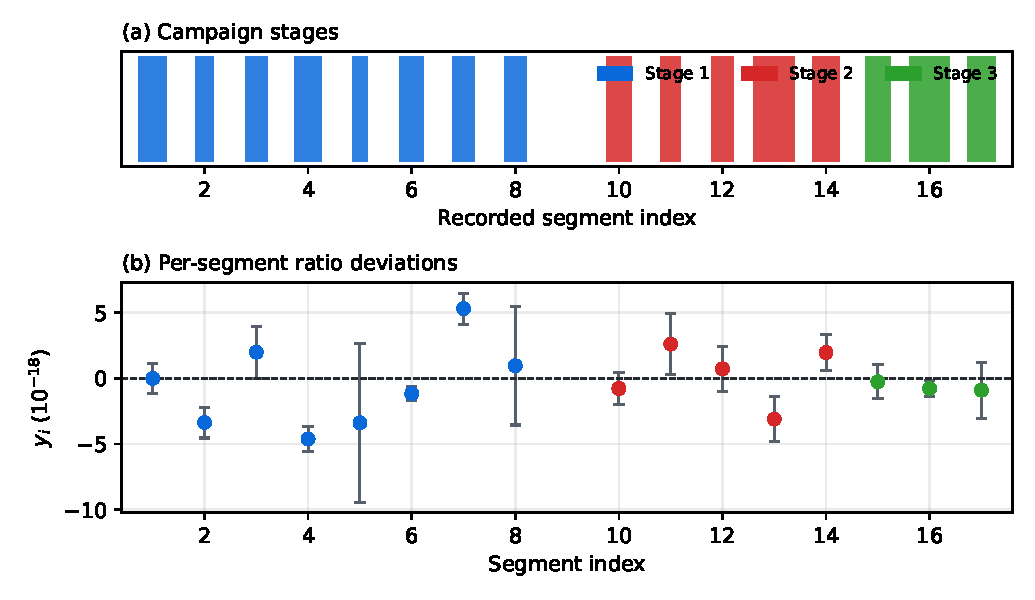
\includegraphics[width=\linewidth]{figs/fig2_campaign.pdf}
  \caption{Campaign and per-segment data. (a) Recorded segments coloured
  by measurement stage; bar widths scale with the square root of the
  retained sample count. (b) Per-segment ratio deviations $y_i$ with
  their statistical uncertainties; the dashed line marks zero deviation.}
  \label{fig:campaign}
\end{figure}

We determine the Yb/Sr frequency ratio from the \nSeg~segments. Each
segment yields a ratio estimate with its own statistical uncertainty
estimated from the Allan deviation of the beat
(Methods). The segment estimates scatter more
than their individual uncertainties allow: the fixed-effect weighted
least-squares fit gives $\chi^2_{\rm red} = \chiRed$ for
$\dofV$ degrees of freedom ($p = \pChi$), and
\nModelLimited~of the \nSeg~segments have stability fits that fall
outside the white-frequency-noise band (groups \modelLimitedGroups).
We therefore adopt the Bayesian random-effect estimate, which treats
the excess scatter as a free parameter and propagates its posterior
uncertainty, while the fixed-effect WLS and Mandel--Paule estimates are
kept as cross-checks.

The resulting Yb/Sr ratio is
\begin{equation}
  \mathrm{Yb/Sr} = \Rheadline(\RheadlineUnc),
\end{equation}
with a statistical uncertainty of
$\uStatShort\times10^{-18}$ and a total standard uncertainty of
$\uTotalShort\times10^{-18}$ (Section~\ref{sec:results-budget}). The
precision-weighted cross-checks agree within their uncertainties:
the WLS centre is \RwlsHead\xspace and the Mandel--Paule centre is
\RmpHead\xspace (rounded at the 19th decimal), both consistent with
the adopted value at the $10^{-18}$ level. Figure~\ref{fig:campaign}b shows the per-segment
deviations; the segment-to-segment scatter is dominated by the
statistical noise of the individual segments and by the excess scatter
captured by the random-effect term.

\subsection{Uncertainty budget}
\label{sec:results-budget}

Table~\ref{tab:budget} collects the components of the total standard
uncertainty (Figure~\ref{fig:compare}b). The statistical term dominates
the budget, followed by the Yb and Sr systematic evaluations, the
static-potential term from the levelling, and the time-varying-redshift
term carried as an uncertainty item; the fibre-link and comb terms are
negligible at this precision. The total standard uncertainty is
$\uTotalShort\times10^{-18}$.

\begin{table}[t]
  \centering
  \caption{Uncertainty budget of the Yb/Sr frequency-ratio
  measurement. The time-varying gravitational-redshift term is carried
  as an uncertainty item and is not applied as a correction to the
  central value. Components are treated as independent.}
  \label{tab:budget}
  \begin{tabular}{lS[table-format=1.3]}
    \toprule
    Component & {Contribution ($10^{-18}$)} \\
    \midrule
    Statistical (Bayesian random effect) & \uStatE \\
    Sr systematics                       & \uSrE \\
    Yb systematics                       & \uYbE \\
    Static gravitational potential       & \uStaticE \\
    Fibre link                           & \uLinkE \\
    Frequency comb                       & \uCombE \\
    Time-varying redshift                & \uTidalE \\
    \midrule
    Total (quadrature)                   & \uTotalE \\
    \bottomrule
  \end{tabular}
\end{table}
